\chapter{Introduction}
\label{cha:introduction}

Learning fundamental behaviour of network data from packet traces is an extremely hard problem. While machine learning (ML) algorithms have been shown as an efficient way of learning from raw data, adapting such algorithms to the general network domain has been hard, to the point that the community doesn't attempt to do so. In our project, we argue that all is not lost, using some specific machine learning architectures like the Transformer, it is indeed possible to develop methods to learn from such data in a general manner.

\section{Motivation}
\label{sec:motivation}

Modelling network dynamics is a \emph{sequence modelling} problem. From a sequence of past packets, we want to estimate the current state of the network (\eg Is there congestion? Will the packet be dropped?), then predict the state's evolution and future traffic's fate --- or which action to take next. Due to the successes in the field of ML and learning from data, it is becoming increasing popular to use such algorithms for solving this modelling problem but the task is notoriously complex. There has been some success in using ML for specific applications in networks, including congestion control\cite{classic,jayDeepReinforcementLearning2019,dynamic,exmachina},
video streaming\cite{oboe,maoNeuralAdaptiveVideo2017,puffer},
traffic optimization\cite{auto},
routing\cite{learnroute},
flow size prediction\cite{flow,onlineflow},
MAC protocol optimization\cite{oneproto,heterowire},
and network simulation\cite{zhangMimicNetFastPerformance2021}, however a good framework for general purpose learning on network data, still doesn't exist.

Today's ML models trained are trained for specific tasks and do not generalize well; \ie they often fail to deliver outside of their original training environments\cite{puffer, datadriven, blackbox}. Due to this, generalizing to different tasks is not even considered. Recent work argues that, rather than hoping for generalization, one obtains better results by training in-situ, \ie using data collected in the deployment environment\cite{puffer}.
Today we tend to design and train models from scratch using model-specific datasets~(Figure \ref{fig:vision}, top). This process is arduous, expensive, repetitive and time-consuming. We always redo everything from scratch in the training process, and never make use of common objectives for training. Moreover, the growing resource requirements to even attempt training these models is increasing inequalities in networking research and, ultimately, hindering collective progress.

As ML algorithms (especially certain deep learning architectures) have shown generalization capabilities\cite{generalizingdnn} in other fields, where an initial \emph{pre-training} phase is used to train models on a large dataset, in a task-agnostic manner and then, in a \emph{fine-tuning} phase, the models are refined on smaller task specific datasets. This helps reuse the general pre-trained model across multiple tasks, making it resource and time efficient. This kind of transfer learning or generalization\cite{transferng} is enabled by using the pre-training phase to learn the overall structure in the data, followed by the fine-tuning phase to focus on learning more task-specific features. As long as there is a certain amount of similarity in the data's structure across the pre-training and fine-tuning, this method can have extremely efficient results.

\section{Tasks, Goals and Challenges}
\label{sec:task}

We argue it is still possible to have learning and generalization in networking. Even if the networking contexts (topology, network configuration, traffic, etc.) can be very diverse, the underlying dynamics of networks remain essentially the same; \eg when buffers fill up, queuing disciplines delay or drop packets. These dynamics can be learned with ML and should generalize and it should not be required to re-learn this fundamental behaviour for training a new model every time. Building such a generic network model for network data is challenging, but this effort would benefit the entire community. Starting from such a model, one would only need to collect a small task-specific dataset to fine-tune it (Figure \ref{fig:vision}, bottom), assuming that the pre-trained model generalizes well. This could even allow modelling rare events (\eg drops after link failures) for which, by definition, only little data is available.

\begin{figure}
    \centering
    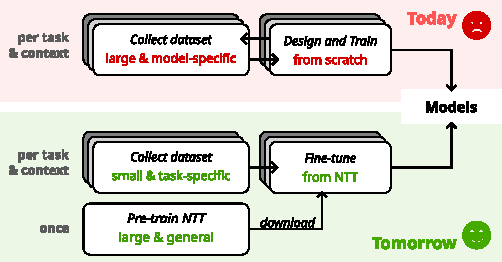
\includegraphics[scale=1.3]{figures/vision}
    \caption{VISION: Collectively learn general network traffic dynamics \emph{once} and focus on task-specific data collecting and learning  for \emph{many future models?}}
    \label{fig:vision}
\end{figure}

While research shows some generalization in specific networking contexts\cite{jayDeepReinforcementLearning2019}, truly ``generic'' models, which are able to perform well on a wide range of tasks and networks, remain unavailable. This is caused by the fact that we usually do not train on datasets large enough to allow generalization, we only train on task-specific smaller datasets. Sequence modelling for a long time, has been infeasible even with architectures dedicated to sequence modelling, such as recurrent neural networks (RNNs), as they can only handle short sequence and are inefficient to train\cite{factor}. However, a few years ago, a new architecture for sequence modelling was proposed: the \emph{Transformer}\cite{vaswaniAttentionAllYou2017} and this proved to be ground-breaking for sequence modelling. This architecture is designed to train efficiently, enabling learning from massive datasets and unprecedented generalization. In a \emph{pre-training phase}, the transformer learns sequential ``structures'', \eg the structure of a language from a large corpus of texts. Then, in a much quicker \emph{fine-tuning phase}, the final stages of the model are adapted to a specific prediction task (\eg text sentiment analysis). Today, Transformers are among the state-of-the-art in natural language processing (NLP\cite{recentnlp}) and computer vision (CV\cite{cvsurvey}).

The generalization power of the Transformer, stems from its ability to learn ``contextual information'', using context from the neighbouring elements in a sequence, for a given element in the same sequence\cite{devlinBERTPretrainingDeep2019}.\footnote{Consider the word \emph{left} in two different contexts: I \emph{left} my book on the table. Turn \emph{left} at the next crossing. The transformer outputs for the word \emph{left} are different for each sequence as they encode the word's context.}
We can draw parallels between networking and NLP. In isolation, packet metadata (headers, etc.) provides limited insights into the network state, we also need the \emph{context}, \ie which we can get from the recent packet history.\footnote{Increasing latency over history indicates congestion.} Based on these parallel, we propose that a Transformer based architecture can also be design to generalise on network packet data. 

Naively transposing NLP or CV transformers to networking fails, as the fundamental structure and biases\cite{biases} in the data are different. Generalizing on complex interactions in networks is not a trivial problem. We expect the following challenges for our Transformer design.

\begin{itemize}
    \item
          How to adapt Transformers for learning on networking data?
    \item
          How to assemble a dataset large and diverse enough to allow useful generalization?
    \item
          Which pre-training task would allow the model to generalize, and how far can we push generalization?
\end{itemize}

\section{Overview}
\label{sec:overview}

We present in our thesis, a Network Traffic Transformer (NTT), which servers a first step, to design a Transformer model for learning on network packet data. We outline the following main technical contributions in this thesis:

\begin{itemize}
\item We present the required background on Transformers, which gives directions to our design, in Chapter \ref{cha:background}.
\item We present the detailed design ideas behind our proof-of-concept NTT in Chapter \ref{cha:design}.
\item We present a detailed evaluation on pre-training and fine-tuning our first NTT models in Chapter \ref{cha:evaluation}.
\item We present several future research directions which can be used to improve our NTT in Chapter \ref{cha:outlook}.
\item We summarise our work and provide some concluding remarks in Chapter \ref{cha:summary}.
\item Supplementary technical details and supporting results are presented in Appendix \ref{app:a} and \ref{app:b}. 
\end{itemize}

A part of the work conducted during this thesis has been submitted as the following paper\cite{newhope} to HotNets '22, and hence, we have some overalap from the the paper's background, design and evaluation sections.

